% 1o trabalho de Cálculo 1
% Questões 13 e 51, cap. 4.7 - problemas de otimização, p. 301-302
% Anderson Fraga - Abril 2023

\documentclass{article}
\usepackage[a4paper,
            includeheadfoot,
            top=2cm,
            right=2cm,
            bottom=3cm,
            left=3cm]{geometry}
\usepackage[OT1]{fontenc}
\usepackage{parskip}
\usepackage{enumitem}
\usepackage{pifont}
\usepackage{tikz}
\usetikzlibrary{calc, shapes}
\usepackage{amssymb}
\usepackage{amsmath}
\usepackage{hyperref} % cria os links de referencia das equacoes

\begin{document}

\underline{\textbf{Resolução do Trabalho 1 de Cálculo I}}\par
\textbf{Sistemas de Informação}\\
\textbf{Instituto Federal do Espírito Santo}\\
Campus Serra\par
\textbf{Cálculo I}\\
Prof. Dr. Fábio Lima\par
Anderson A. Fraga (20222BSI0482)\\
\texttt{aafrg@tuta.io}\\  %\texttt formats the text to a typewriter style font

\noindent \underline{\textbf{Cap. 4.7 - Problemas de otimização}}\par
\noindent \textbf{Questão 13) Um fazendeiro quer cercar uma área de 15.000 $m^2$ em um campo retangular e então dividi-lo ao meio com uma cerca paralela a um dos lados do retângulo. Como fazer isso de forma que minimize o custo da cerca?}\par
Para determinar a melhor opção para a construção de uma cerca paralela a um dos lados do campo, representado na Figura 1, pode-se definir que:
\begin{enumerate}[label=(\roman*)]
    \item Dois dos lados do campo terão comprimentos iguais $(a)$ e três outros também terão lados iguais, $(b)$, já que é um campo \underline{retangular} e que será dividido ao meio;
    \item Que a área do campo é definida como $A_{campo} = a \times b$ e que necessariamente tem que ser igual a 15.000 $m^2$;
    \item O custo da cerca será diretamente proporcional ao perímetro adotado; e que este perímetro pode ser definido por $P_{campo} = a + a + b + b + b \therefore P_{campo} = 2a + 3b$;
\end{enumerate}
Assim, delimita-se geometricamente o campo como:
\begin{figure}[!h] % necessario inserir a tikzpicture dentro da figure para centralizar
    \centering
    \begin{tikzpicture}
        \draw [anchor=center] (0,1) node[minimum width=3cm, minimum height=2cm, draw] {}; % para transformar em retangulo, adicionar minimum width=3cm e minimum height=2cm, p.e.
        \draw[anchor=center] (-1.8,1) node{b} (-0.3,1) node{b} (1.7,1) node{b}; % lado b
        \draw[anchor=base]   (0,2.3) node{a} (0,-0.5) node{a}; % lado a
        \draw[anchor=base]   (0,2) node{} -- (0,0) node{}; % linha divisoria do campo
    \end{tikzpicture}
    \caption{Exemplo geométrico do campo retangular}
\end{figure}
\par Ao desenvolver $(i)$ utilizando $(ii)$, isola-se uma das variáveis para simplficar a otimização. Desta forma, temos que:
\begin{eqnarray}
    \label{eq:1.1}
    A_{campo} & = &a \times b \nonumber\\
    1500 & = &a \times b \nonumber\\
    b & = &\frac{15000}{a}
\end{eqnarray}
Substituindo $b$ de $(ii)$ em $(i)$, o perímetro $P_{campo}$ resulta em:
\begin{eqnarray}
    \label{eq:1.2}
    P_{campo}   & = &2a + 3b \nonumber\\
    & = &2a + 3 \times \frac{15000}{a} \nonumber\\
    & = &2a + 45000*{a^{-1}}
\end{eqnarray}
A otimização, neste caso, exige a descoberta dos pontos críticos que envolvem a dimensão do campo em questão. Desta forma, determina-se os pontos críticos em função da Equação \ref{eq:1.2}, como demonstrado abaixo.
\begin{eqnarray}
    \label{eq:1.3}
    P_{campo}   & = & 2a + 45000 \times {a^{-1}} \nonumber\\
    P'_{campo}   & = & 2 + 45000 \times -1 \times a^{-2} \\
    & = & 2 + 45000 \times -1 \times a^{-2} \nonumber\\
    2 & = & 45000 \over a^{2} \nonumber\\
    a^{2} & = & 45000 \over 2 \nonumber\\
    a^{2} & = & 22500 \nonumber\\
    a & = & \sqrt[]{22500} \nonumber\\
    a & = & \pm 150 \nonumber
\end{eqnarray}
Como não existe medida negativa, despreza-se o valor negativo encontrado na derivada de $\mathbf{a}$ na Equação \ref{eq:1.3}.
Retornando na Equação \ref{eq:1.1}, calcula-se o valor de $\mathbf{b}$ substituindo $\mathbf{a}$:
\begin{eqnarray}
    \label{eq:1.4}
    b & = &\frac{15000}{a} \nonumber\\
    b & = &\frac{15000}{150} \nonumber\\
    b & = &100 \nonumber
\end{eqnarray}
Assim, as dimensões ótimas para a construção da cerca em torno do campo dividido são $\mathbf{a = 150m}$ e $\mathbf{b = 100m}$.

\noindent \textbf{Questão 51) A iluminação de um objeto por uma fonte de luz é diretamente proporcional à potência da fonte e inversamente proporcional ao quadrado da distância da fonte. Se duas fontes de luz, uma três vezes mais forte que a outra, são colocadas a 4 m de distância, onde deve ser colocado o objeto sobre a reta entre as fontes de forma a receber o mínimo de iluminação?}\par
Admitindo que:
\begin{enumerate}[label=(\roman*)]
    \item Existem duas distâncias iniciais, $d$ e $4-d$, entre a fonte de luz, $l$, e o objeto;
    \item Esquematizando os itens apresentados no problema, as posições dos elementos podem ser interpretadas da sequinte forma:
          \begin{figure}[!h]
              % https://tikz.dev/tikz-graphscentralizar
              \centering
              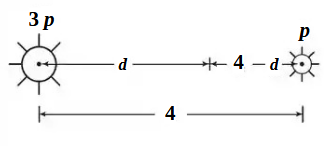
\includegraphics[scale=.85]{fig51.png}
          \end{figure}
    \item Podemos classificar as duas fontes de luz segundo sua potência de iluminação, $p$, como:
          \begin{itemize}
              \item[\ding{220}] $l_1$, com potência igual a $3p$; e % https://latex-tutorial.com/tutorials/lists/; https://latex-tutorial.com/wp-content/uploads/2021/12/Bullet-styles-pifonts-1024x790.webp
              \item[\ding{220}] $l_2$ com potência igual a $p$.
          \end{itemize}
    \item Podemos, também, relacionar a iluminação do objeto, $i$, a potência da fonte de luz $l_1$ e as distâncias como representado abaixo na Equação \ref{eq:2.1}:
          \begin{equation}\tag{2.1}
              \label{eq:2.1}
              i_1 = {3p \over d^2}
          \end{equation}
    \item Como a relação complementar a esta proporção para $l_2$, onde:
          \begin{equation}\tag{2.2}
              \label{eq:2.2}
              i_2 = {p \over {(4-d)^2}}
          \end{equation}
\end{enumerate}
Assim, somando as relações apresentadas nas Equações \ref{eq:2.1} e \ref{eq:2.2} e considerando que $\mathbf{d}$ estará dentro de um intervalo $\mathbf{0 \leqslant d \leqslant 4}$, temos:
\begin{equation}\tag{2.3}
    \label{eq:2.3}
    i_{total} = {{3p \over d^2} + {p \over {(4-d)^2}}}
\end{equation}
Otimizando $\mathbf{i_{total}}$ por meio da derivação da Equação \ref{eq:2.3} a fim de encontrar o valor crítico para a distância entre as fontes luminosas, tem-se:
\begin{align}
    \label{eq:2.4}
    i'(d)       & = {-{6p \over d^3} + {2p \over {(4-d)^3}}} = 0 \tag{2.4} \\
    6p(4-d)^{3} & = 2pd^{3} \nonumber                                      \\
    3(4-d)^{3}  & = d^{3} \nonumber
\end{align}
Simplificando a Equação \ref{eq:2.4} e retirando a raiz cúbica:
\begin{align}
    \label{eq:2.5}
    \sqrt[3]{3}\sqrt[3]{(4-d)^{3}} & = \sqrt[3]{d^{3}} \nonumber                            \\
    \sqrt[3]{3}(4-d)^{3}           & = d \nonumber                                          \\
    4\sqrt[3]{3}-\sqrt[3]{3}d      & = d \nonumber                                          \\
    d + \sqrt[3]{3}d               & = 4\sqrt[3]{3} \nonumber                               \\
    d(1 + \sqrt[3]{3})             & = 4\sqrt[3]{3} \nonumber                               \\
    d                              & = {{4\sqrt[3]{3}} \over {(1 + \sqrt[3]{3})}} \nonumber \\
    d                              & \approx 2,36m \nonumber
\end{align}
Ao final, temos que se $d$ equivale a $2,36m$ para a fonte de maior iluminação, então $4 - 2,36 = 1,64m$, ou seja, a fonte de menor iluminação precisa estar a $1,64m$ de distância.
\end{document}
